\color{black}
{\color{secblue}\subsection{Purpose}}

{\color{secblue}\subsubsection{General Description}}
The purpose of this section is to highlight some constraints in the model, through a simplified model of alloy.
Three models are described here, one for each service to develop (Data4Help, AutomatedSOS and Track4Run), each with one or more aspect to show:
\begin{itemize}
\item \textbf{Data4Help:} here the model includes users, their data, third parties and query and requests, and the focus is on these last two. In particular two predicates are showed, one considering a world with queries but without requests and the opposite for the other. In the query example world the focus is on the validity of a query, meaning the number of results provided is high enough to return it to the TP which requested it. Also a global query is shown, meaning a query which returns all registered user's datas. Is present an assertion which checks that a global query actually returns all the userdatas present in the model.
\item \textbf{AutomatedSOS:} AutomatedSOS consists in a simple model, composed by Devices (implicitly bound to a user, which is not included because not relevant here), Calls and ValuesLists, which represent all the values taken by a specific device in a precise moment in time. The focus is set on the time-critical operation of the call to the ospital, which must be made by the device at the first moment the values of the user reach a dangerous point, and not before or after that moment. Another case shown is the absence of calls in case of safe conditions. Is also made an assertion on the fact that at most one call per device is made in this model.
\item \textbf{Track4Run:} this last model aims to show the interaction between elements of the application. here are modeled users, runs and registration to them, with a particular focus on users' possibilities and permissions. The two examples show different aspect of the Track4Run system. In the first one is shown a user who is both a creator and a participant, and in the second is shown a user which is visible in a certain time, because he's participating in a run at that time, and not visible in another time.
Finally is made an assertion on the visibility of a user which is not a participant: such user cannot be visible at any time.
\end{itemize}

{\color{secblue}\subsubsection{Simplifications}}
All of the following semplifications are meant to simplify the models and/or reduce complexity of generated example worlds, without loss of meaning relatively to the focus of each one.
By doing simplifications, some integer values are not related strictly to the meaning of their variable, but should be seen instead as a symbolic partition of the real range of the variables.

\paragraph{Data4Help}
\begin{itemize}
\item Position of a user is of type (x,y) and x,y are bounded [0,2]
\item Age of a user is bounded [0,5]
\item Queries can group by only equality (not inclusion in range)
\item UserData includes only position, age and gender
\item Queries are returned when there are at least 3 users in the result, instead of 1000
\item Queries return user data not without filtering: in the model the privacy is not considered.
\end{itemize}

\paragraph{AutomatedSOS}
\begin{itemize}
\item Values taken in ValuesLists are only pressure, temperature and heartbeat, to set an example.
\item All the values in ValuesLists are bounded [0,5]
\item Timestamps are bounded [0,2]
\item The model shows always exactly 3 values lists per device, to simulate 3 consecutive points in time where values were taken
\item The model shows a single case of an emergency situation, resulting in the fact that no more than one call can be made, because the subsequent calls would be pointless
\end{itemize}

\paragraph{Track4Run}
\begin{itemize}
\item Time is represented generically with a Time signature. It stands for an abstract amount of time, depending on the run, in which a run can be held (e.g. a couple of hours).
For simplicity and abstraction Time is not specified as a date or with a unit of measure
\item Runs have at least 2 partecipants
\item Tracks are defined by a set of generic MapPoints, containing at least 2 of them
\item Real time maps have an internal date which indicates when the partecipants are seen by spectators on the map
\item VisibleUsersInACertainTime are signatures which indicate which users can be seen through the app in a specific time. This information is not related with any user in particular (i.e. cannot happen that one user can see more participants than another at the same time) because any user can watch a run, so a participant position is accessible by any user during the run
\end{itemize}
\newpage
{\color{secblue}\subsection{Code}}
{\color{secblue}\subsubsection{Data4Help}}
\lstset{frame=tb,
  language=Java,
  aboveskip=3mm,
  belowskip=3mm,
  showstringspaces=false,
  columns=flexible,
  basicstyle={\small\ttfamily},
  numbers=none,
  numberstyle=\tiny\color{gray},
  keywordstyle=\color{blue},
  commentstyle=\color{dkgreen},
  morekeywords={sig, one, Int, and, open, abstract, extends, set, lone, fact, all, disj, some, in, implies, iff, assert, pred, check, run, for, but},
  breaklines=true,
  breakatwhitespace=true,
  tabsize=3
}
\lstinputlisting{./alloy/data4help.als}
\newpage
{\color{secblue}\subsubsection{AutomatedSOS}}
\lstset{frame=tb,
  language=Java,
  aboveskip=3mm,
  belowskip=3mm,
  showstringspaces=false,
  columns=flexible,
  basicstyle={\small\ttfamily},
  numbers=none,
  numberstyle=\tiny\color{gray},
  keywordstyle=\color{blue},
  commentstyle=\color{dkgreen},
  morekeywords={sig, one, Int, and, open, abstract, extends, set, lone, fact, all, disj, some, in, implies, iff, assert, pred, check, run, for, but},
  breaklines=true,
  breakatwhitespace=true,
  tabsize=3
}
\lstinputlisting{./alloy/automatedSOS.als}
\newpage
{\color{secblue}\subsubsection{Track4Run}}
\lstset{frame=tb,
  language=Java,
  aboveskip=3mm,
  belowskip=3mm,
  showstringspaces=false,
  columns=flexible,
  basicstyle={\small\ttfamily},
  numbers=none,
  numberstyle=\tiny\color{gray},
  keywordstyle=\color{blue},
  commentstyle=\color{dkgreen},
  morekeywords={sig, one, Int, and, open, abstract, extends, set, lone, fact, all, disj, some, in, implies, iff, assert, pred, check, run, for, but},
  breaklines=true,
  breakatwhitespace=true,
  tabsize=3
}
\lstinputlisting{./alloy/track4run.als}

\newpage
{\color{secblue}\subsection{Worlds Generated}}
{\color{secblue}\subsubsection{Data4Help}}
\begin{figure}[H]
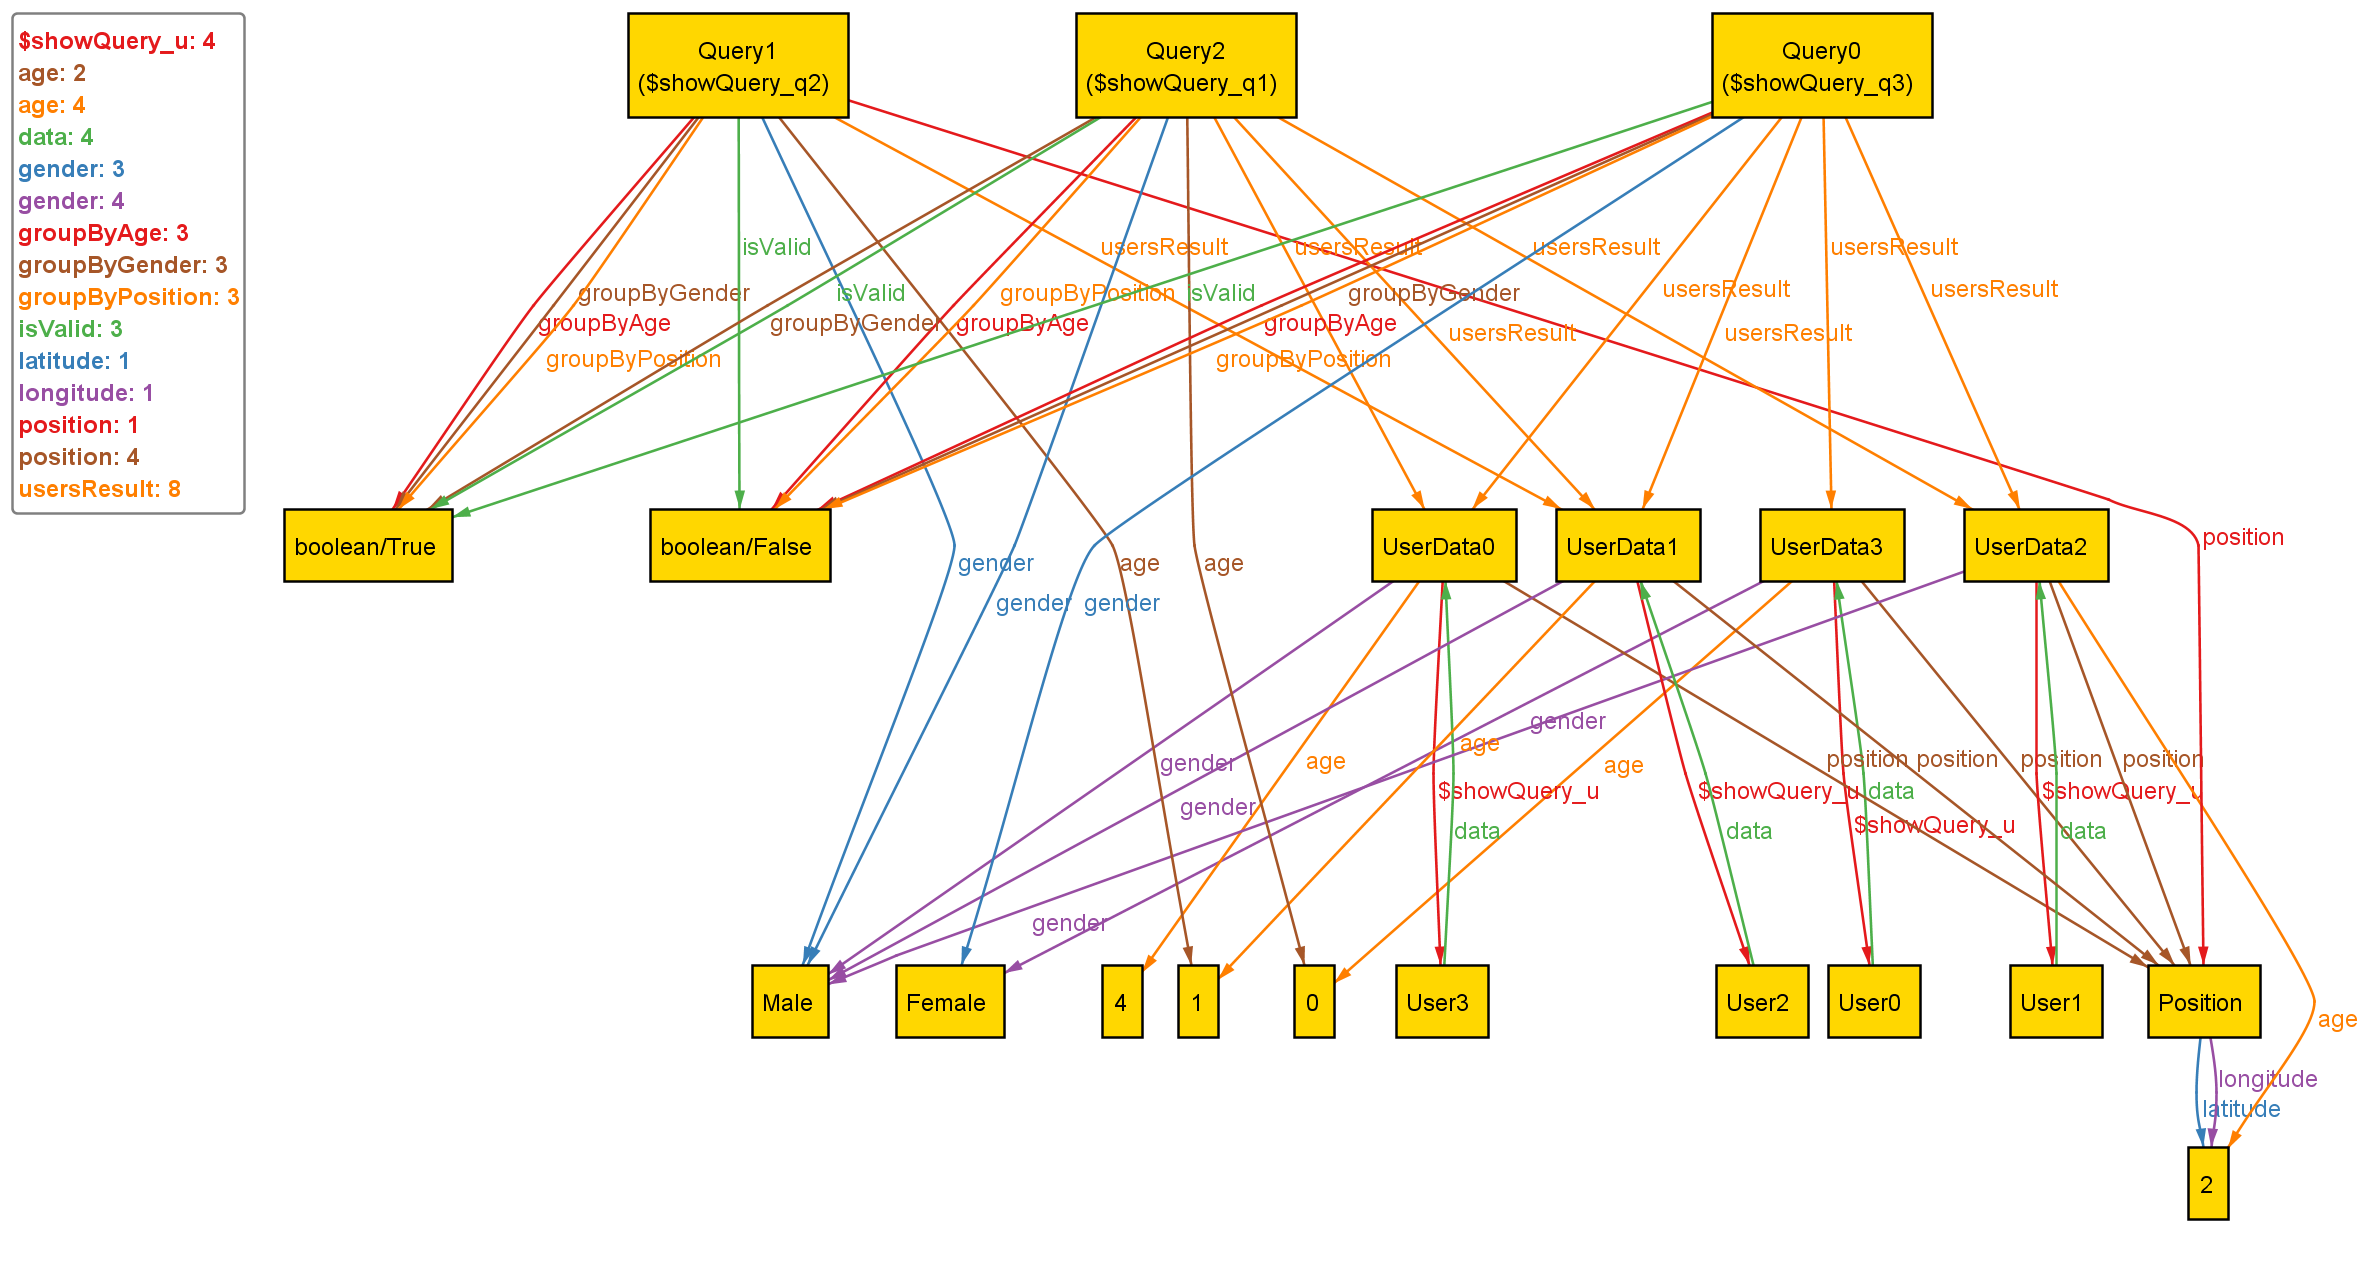
\includegraphics[height=10cm, keepaspectratio]{./Images/Alloy/data4help_1.png}
\centering
\caption{Data4Help case 1: q1 is a valid query, q2 is a non-valid query, q3 is a global query}
\end{figure}
\begin{figure}[H]
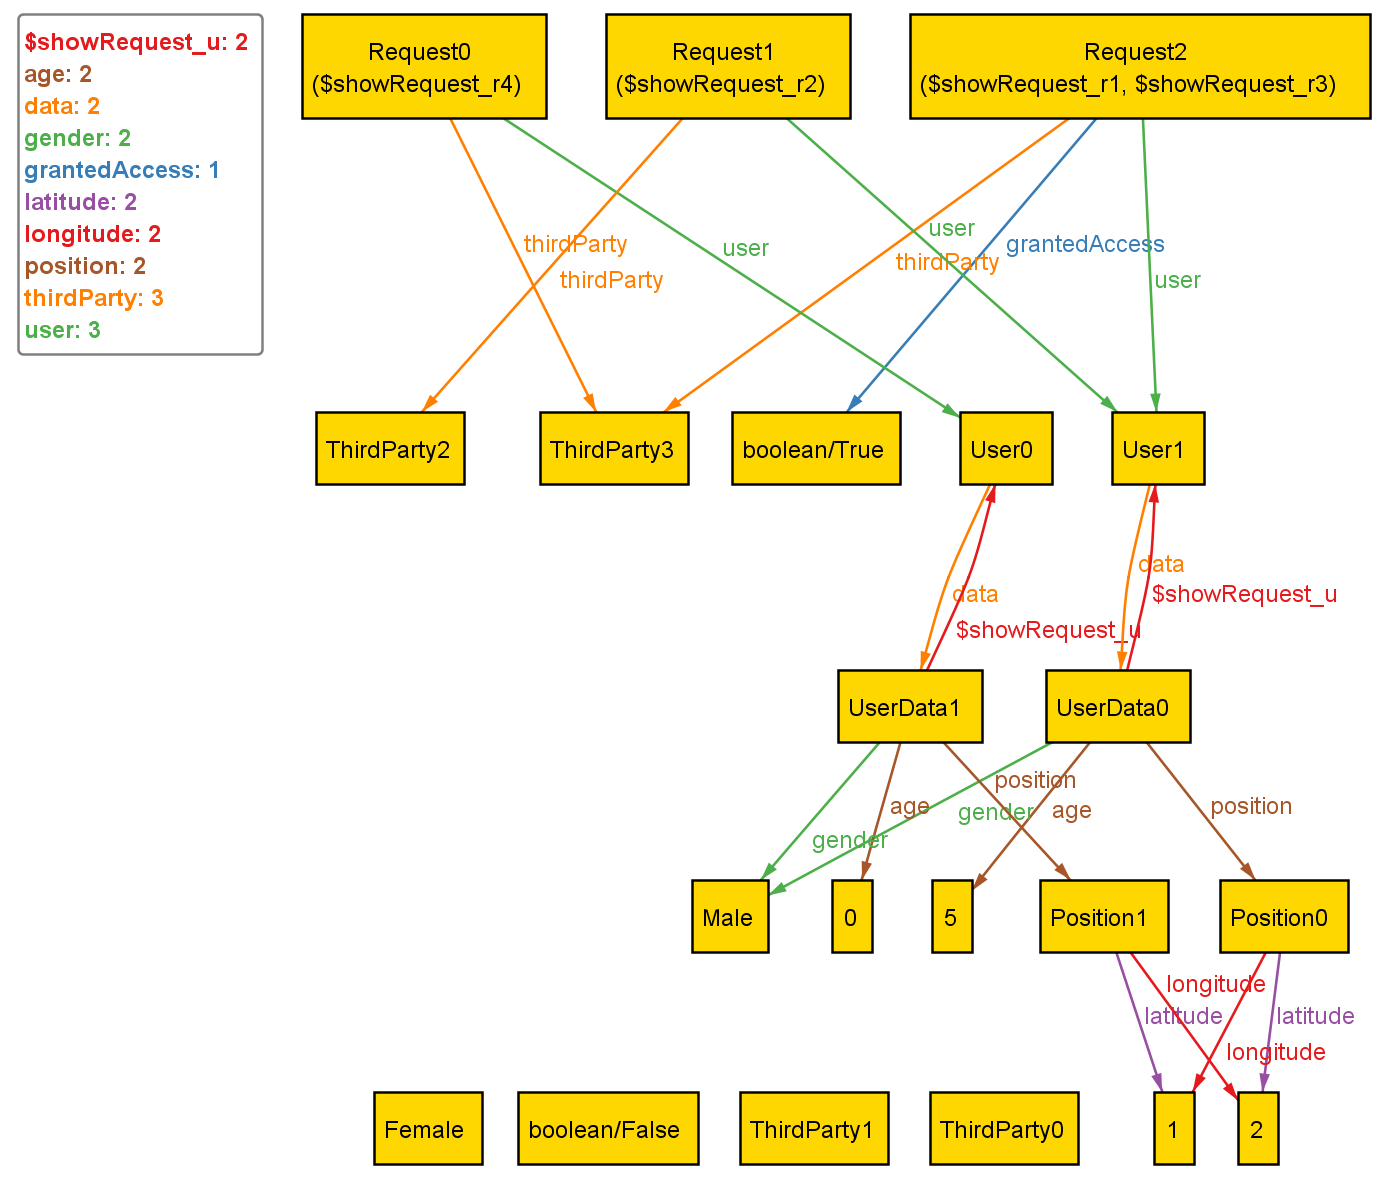
\includegraphics[width=\linewidth, height = 9cm, keepaspectratio]{./Images/Alloy/data4help_2.png}
\centering
\caption{Data4Help case 2: r1 and r2 are requests with same user, but 1 is accepted and the other is not. r3 and r4 are requests made by the same TP, one accepted and the other not}
\end{figure}

\newpage
{\color{secblue}\subsubsection{AutomatedSOS}}
\begin{figure}[H]
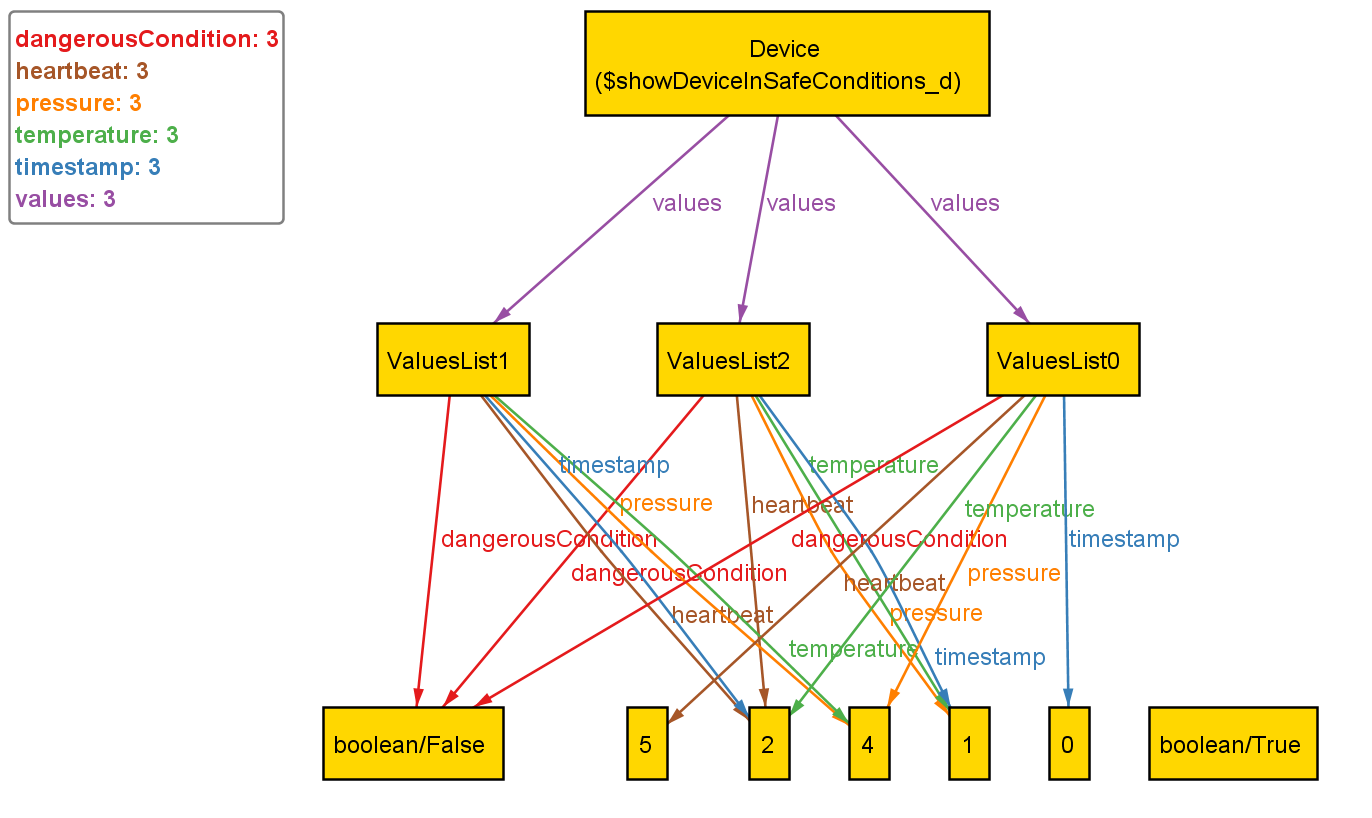
\includegraphics[width=\linewidth]{./Images/Alloy/automatedSOS_1.png}
\centering
\caption{Automated SOS case 1: a device which never registers dangerous conditions}
\end{figure}
\begin{figure}[H]
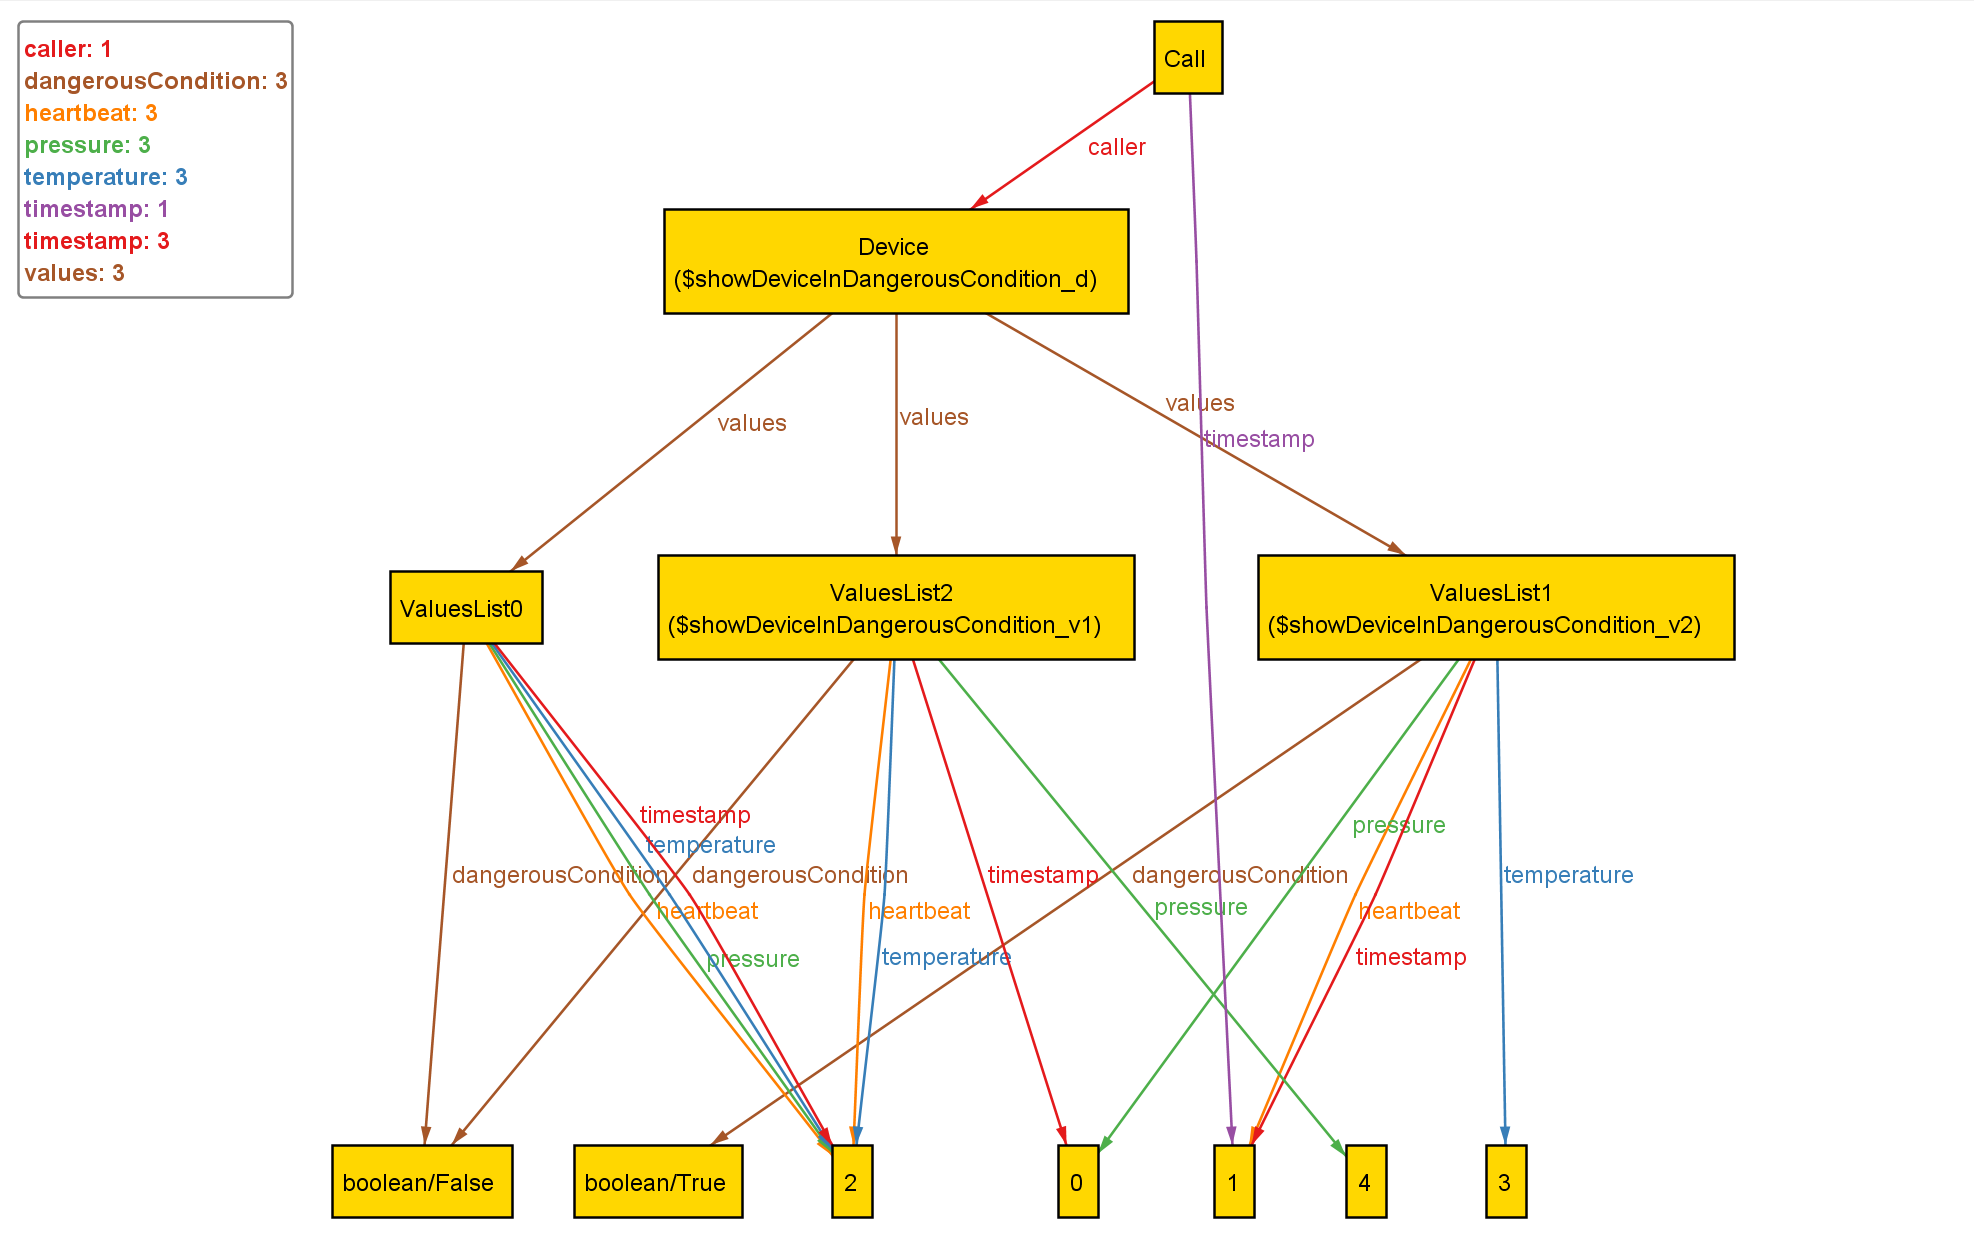
\includegraphics[width=\linewidth]{./Images/Alloy/automatedSOS_2.png}
\centering
\caption{Automated SOS case 2: a device which registers a dangerous condition starting from timestamp 1, having so a call at the same timestamp}
\end{figure}

\newpage
{\color{secblue}\subsubsection{Track4Run}}
\begin{figure}[H]
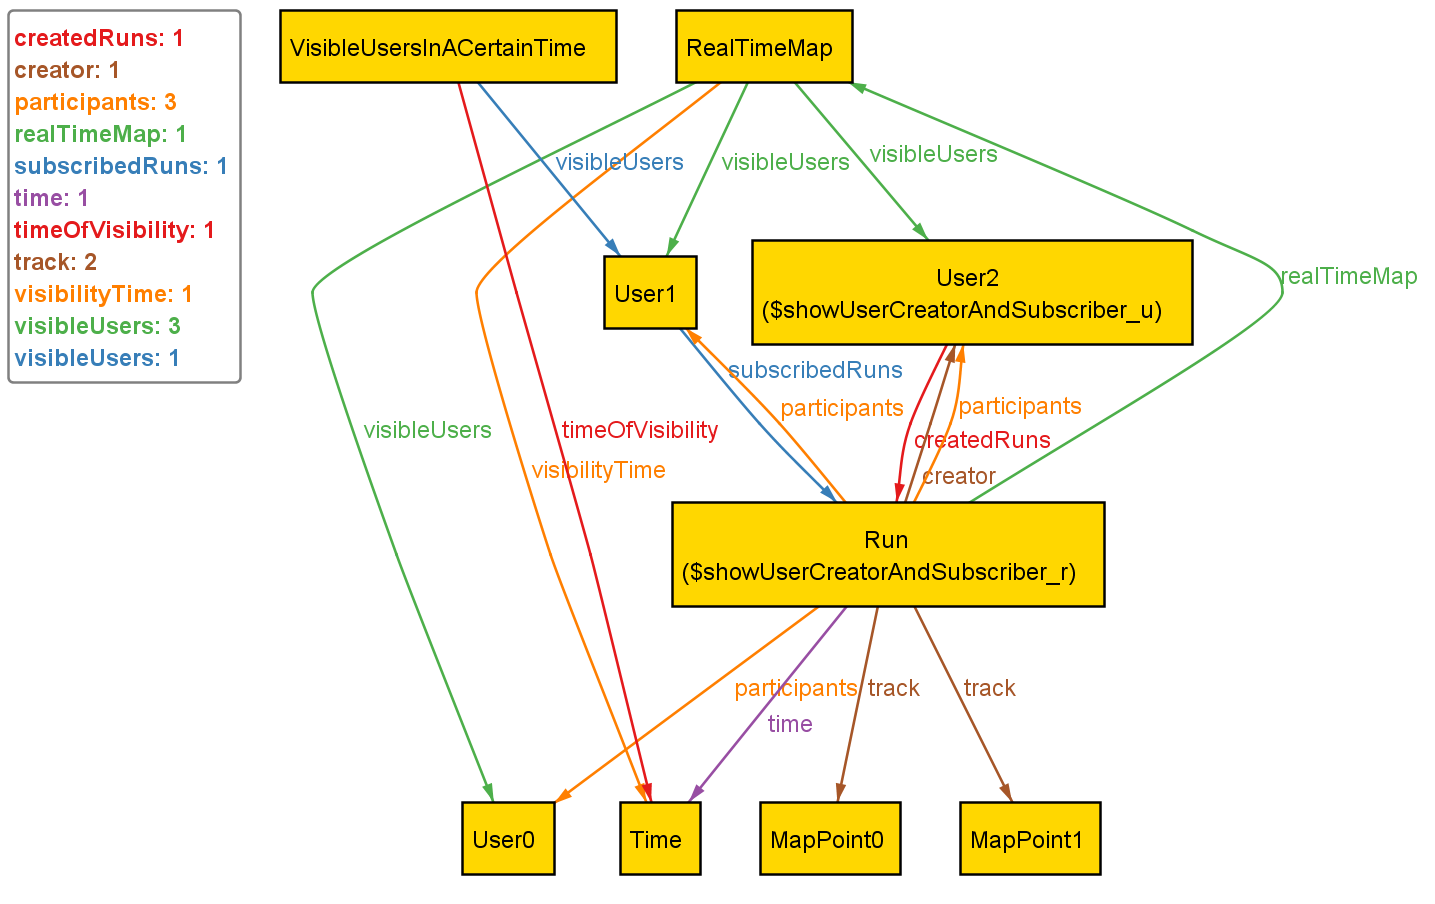
\includegraphics[width=\linewidth, height=8cm, keepaspectratio]{./Images/Alloy/track4run_v2_1.png}
\centering
\caption{Track4Run case 1: user u (User2) is at the same time the creator and a participant in the same run}
\end{figure}

\begin{figure}[H]
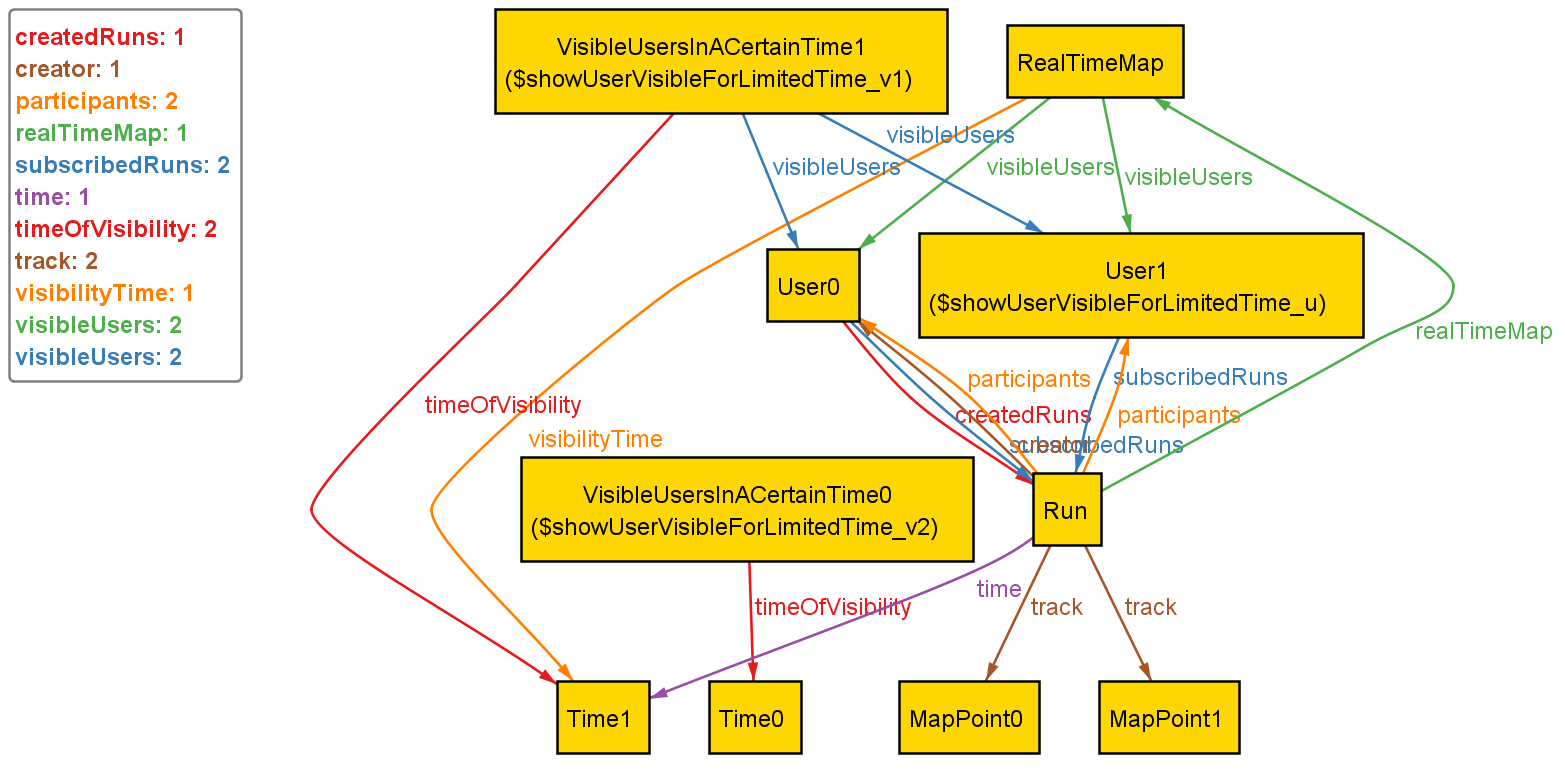
\includegraphics[width=\linewidth, height=10cm, keepaspectratio]{./Images/Alloy/track4run_v2_2.png}
\centering
\caption{Track4Run case 2: user u (User1) is visible in a certain time (Time1) but not in another (Time 0)}
\end{figure}
\newpage
{\color{secblue}\subsection{Alloy results}}
\begin{figure}[H]
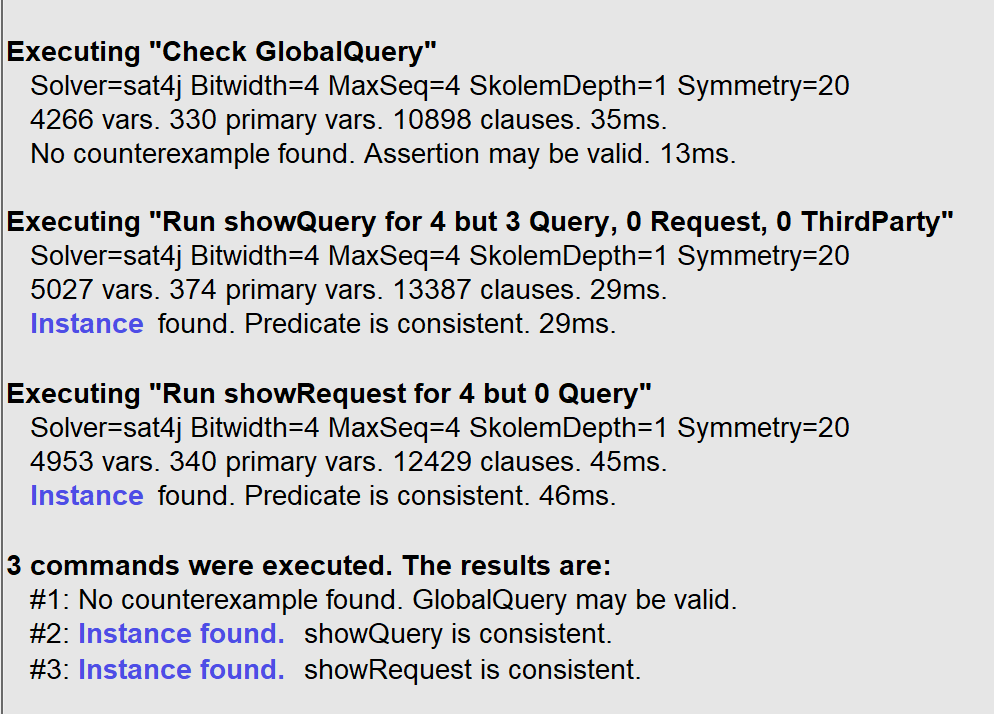
\includegraphics[width=\linewidth, height=6cm, keepaspectratio]{./Images/Alloy/data4help_results.png}
\centering
\caption{Data4Help's alloy results}
\end{figure}

\begin{figure}[H]
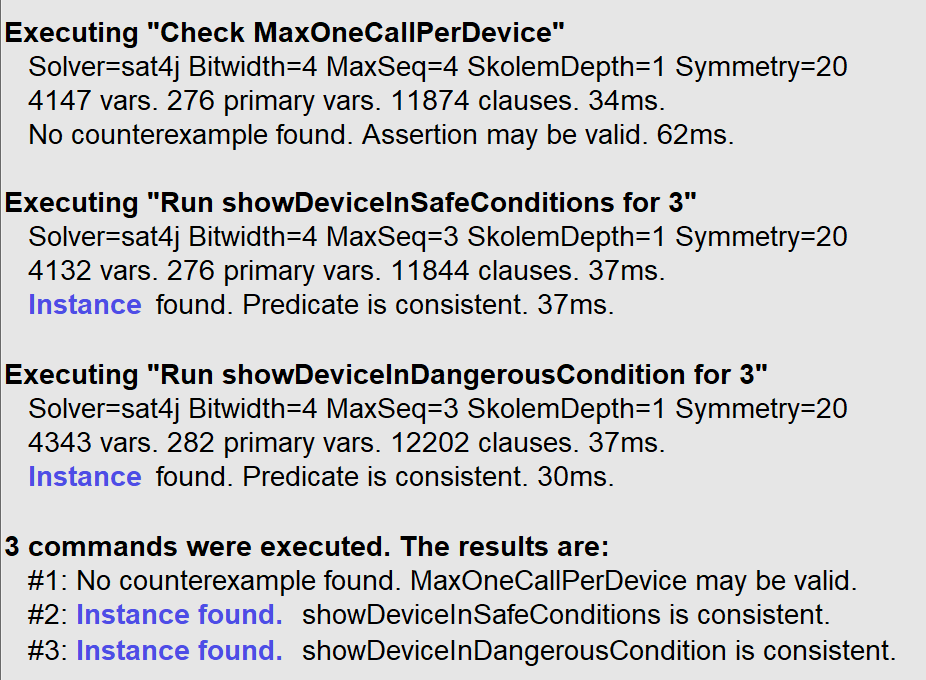
\includegraphics[width=\linewidth, height=6cm, keepaspectratio]{./Images/Alloy/automatedSOS_results.png}
\centering
\caption{AutomatedSOS' alloy results}
\end{figure}

\begin{figure}[H]
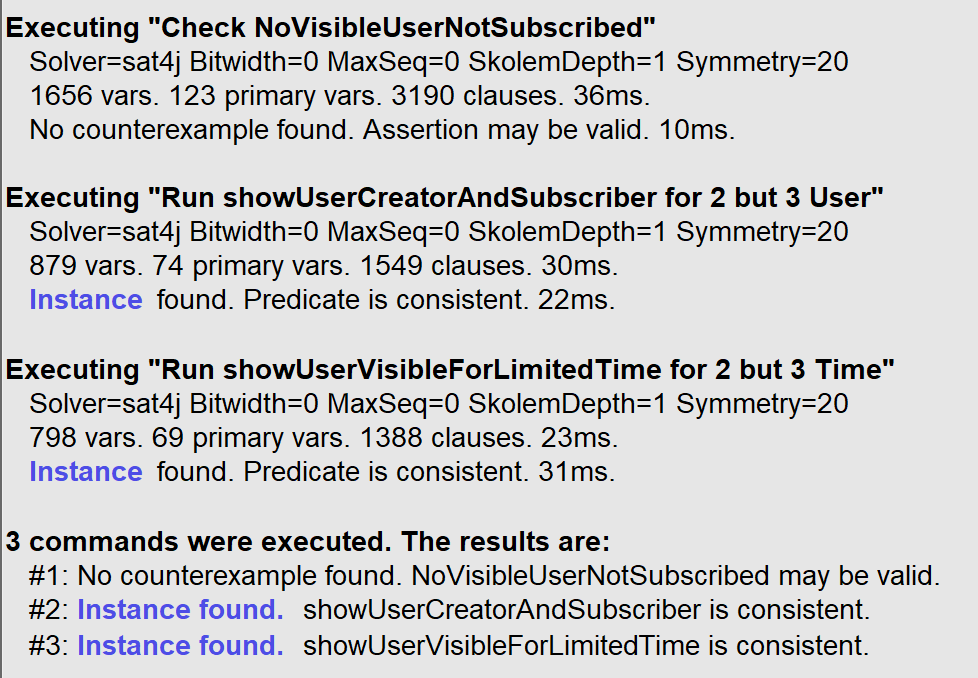
\includegraphics[width=\linewidth, height=6cm, keepaspectratio]{./Images/Alloy/track4run_v2_results.png}
\centering
\caption{Track4Run's alloy results}
\end{figure}